\documentclass[twoside]{article}
\usepackage{enumitem}
\usepackage{textcomp}
\usepackage[table]{xcolor}
\usepackage{xcolor}
\usepackage[latin9]{inputenc}
\usepackage{booktabs}
\usepackage{mathtools}
\usepackage{multirow}
\usepackage{enumitem}                 
\usepackage{amsmath}
\usepackage{amsthm}
\usepackage{amssymb}
\usepackage{graphicx}




\input{ISC18-english.sty}
%%%%%%%%%%%%%%%%%%%%%%%%%%%%  Make sure to compile twice for proper cross-references. %%%%%%%%%%%%%%%%%%%%%%%
%%%%%%% For proper display of references, compile the document twice. %%%%%%%%%%%%%%%%%%%%% 
%%%%%%%%%%%%%%% If using TeX Live, compile using pdflatex command %%%%%%%%%%%%%%%%%%%%%%%
\begin{document}
\thispagestyle{empty}
%%%%%%%%%%%%%%%%% Article title header  %%%%%%%%%%%%%%%%%%%%
\fancyhead[LE]{MRL Estimation Using NRSS}
%%%%%%%%%%%%%%%%% Article authors header   %%%%%%%%%%%%%%%%%%%%
\fancyhead[RO]{Jabari and Zamanzade}
\begin{center}
{
\includegraphics [height=25mm, width=150.3mm] {Images/isc18E}} \\
\vspace*{-1.8cm}
%\begin{center}
%\color{blue} 
%{\hspace{0.1cm}\rule{\textwidth}{1mm}}\\
%\end{center}
\vspace*{4cm}
%%%%%%%%%%%%%%%%% Article title  %%%%%%%%%%%%%%%%%%%%
{\Large \bf Estimation of the Mean Residual Life Function Using Neoteric Ranked Set
	Sampling}\\
%%%%%%%%%%%%%%%%% Article authors and affiliations %%%%%%%%%%%%%%%%%%%%
{\bf
Leila Jabari Koopaei$^1$ \footnote[2]{{\bf Corresponding Author: } {\tt  leilajabari1394@gmail.com; l.jabari@vru.ac.ir. }}, Ehsan Zamanzade$^2$   \\
$^1$Department of Statistics, Vali-e-Asr University of Rafsanjan, Rafsanjan, Iran.  \\
$^2$Department of Statistics, Faculty of Mathematics and Statistics,
University of Isfahan, Isfahan, Iran.}
\end{center}
\rule{\textwidth}{0.2mm}\\
%%%%%%%%%%%%%%%%% Article abstract  %%%%%%%%%%%%%%%%%%%%
\noindent{\bf Abstract:}\\
 The mean residual life (MRL) function is one of the fundamental concepts in survival analysis. The MRL is easily interpretable and particularly useful for conveying the survival information to patients.  Ranked set sampling
(RSS) is a sampling design useful for situations where precise quantification of units is
costly or difficult, but ranking them based on associated variables is easy with negligible cost. In recent years, different modifications
of RSS have been introduced to enhance its efficiency. This paper investigates the estimation
of the MRL function using Neoteric Ranked Set Sampling (NRSS), a notable modification of
RSS. We compare the proposed estimator with its counterparts in RSS and SRS using Monte
Carlo simulation. Our results show that the proposed estimator is more efficient than its
counterparts  for small and moderate sample sizes. 

\noindent{\bf Keywords:} 
Mean residual life, Neoteric ranked set sampling, Monte Carlo simulation, Ranked set sampling.  \\
\noindent{\bf Mathematics Subject Classification (2010):} $\rm 62D05$, $\rm 62G05$. \\
\hspace{1cm}\rule{\textwidth}{0.2mm}\\
%%%%%%%%%%%%%%
\section{Introduction}
Suppose $X$ is a continuous random variable, with $F \left(0\right) =0$ and $\mu= \mathbb{E}\left( X \right)=\int_{0}^{\infty }S\left( x \right)dx< \infty $. The mean residual lifetime function at time
$t\geq0$ is defined as 
\begin{equation}
	m(t)=\mathbb{E}\left(X-t|X>t\right)=\frac{{\int_{t}^{\infty}{S(x)dx}}}{{S(t)}},\label{eq_m}
\end{equation}
provided that $S(t)>0$, and $m\left(t\right)=0$ whenever $S\left(t\right)=0$. Note that $m\left(0\right)=\mu$.

The MRL function is important in various application areas such as reliability engineering, medicine, and actuarial science. Like the survival or hazard functions, this function uniquely characterizes the distribution, making it interesting to statisticians. However, unlike the survival or hazard functions, it summarizes the effect of a treatment or a risk factor in time units instead of on a probability scale. This makes it easily interpretable and of interest to many non-statistician scientists.

In some scientific fields, such as agriculture, healthcare, environmental, and ecological studies, measuring the variable of interest might require expensive equipment or long-term studies. However, ranking a few of them based on professional judgment or associated auxiliary variables is not difficult and involves negligible cost. Ranked set sampling (RSS), a sampling technique introduced by \cite{McIntyre(1952)}, is suitable for these situations. Several studies have shown that RSS can be more efficient than SRS for estimating a wide range
of population parameters, including the mean \citep{Frey2012}, proportion \citep{Zamanzade2020}. 

One of the challenges of using RSS instead of SRS is the potential for errors in ranking observations.
In recent years, several modifications and extensions of RSS have been proposed in the
literature to reduce ranking errors and improve the efficiency of the population mean estimator.  \cite{Zamanzade2016} proposed the neoteric ranked set sampling (NRSS) and showed its relative efficiency improvements in estimating the population mean and variance.

In survival analysis, accurately measuring the variable of interest sometimes requires expensive
equipment or long-term follow-up. In these cases, cost-effective sampling methods, such as RSS
or its modifications, are desirable because they can reduce the required sample size while still
achieving the desired level of precision. Recently, several studies have been conducted on the
fundamental functions of survival analysis based on RSS.  \cite{Strzalkowska2014}  proposed the Kaplan-Meier estimator of survival function based on RSS
under random censored data. \cite{Zamanzade2019} addressed the problem of estimating
the MRL in RSS.

In Section \ref{Sec2}, we describe the basic definitions of  RSS and NRSS techniques. 
In Section \ref{Sec3}, we discuss the estimation of the MRL function based on NRSS technique. Section \ref{Sec4} presents our simulation study comparing the performance of the MRL estimator using NRSS with its SRS and RSS counterparts. 

\section{  Sampling Procedures for RSS and NRSS} \label{Sec2}
In this section, we provide a detailed description of how to draw samples using RSS and NRSS.
To obtain a balanced RSS  with a total sample size of $n = m \times r$, where $m $ (set size)  and $r$ (cycle size) must be determined before sampling,  we select a random sample of size $m^2$ elements from the population of interest, which is then partitioned into $m$ sets of $m$ units. Then, we rank each set from smallest to largest,  either virtually or by any cost-effective method.  Actual measurements are taken only on the $i$th smallest units in each $i$th set, where $i=1,\dots,m.$ The procedure can be reiterated $r$ times to yield a sample with a size of $n = m \times r$. The final sample is denoted as $  \{ {X_{[i]j}},{\rm{ }}i = 1,\dots,m;{\rm{    }}j = 1,\dots,r\}  $, where $ X_{[i]j}$ is the $i$th ordered judgment unit in the $j$th cycle.  

To obtain an NRSS sample of size $n=m\times r$, similar to RSS,  we must first determine the set size $m $ and cycle size $r$, then select $m^2$ simple random samples from the population. Then, we rank the $m^2$ samples from smallest to largest,  either virtually or by any cost-effective method.  Actual measurements are taken only on the $\left[l+\left(i-1\right)m \right]$th smallest units in the set, for $i=1,\dots,m$, where:
	\vspace{-1.5ex}  
	\begin{itemize}[itemsep=-1ex] 
		\item \( l = \frac{m+1}{2} \) if \( m \) is odd,
		\item \( l = \frac{m}{2} \) if both \( m \) and \( i \) are even,
		\item \( l = \frac{m}{2}+1 \) if \( m \) is even but \( i \) is odd.
	\end{itemize}
 The procedure can be reiterated $r$ times to yield a sample with a size of $n = m \times r$.
The final sample is represented as $  \{ {X_{\left[l+\left(i-1\right)m \right]j}},{\rm{ }}i = 1,\dots,m;{\rm{    }}j = 1,\dots,r\}  $, where $ X_{\left[l+\left(i-1\right)m \right]j}$ is the $[l+\left(i-1\right)m]$th ordered judgment unit in the $j$th cycle. 
To better understand how NRSS works and compare it with RSS, we illustrate the construction of one RSS sample with a set size of $m = 3$ and a cycle size of $r = 2$, along with two NRSS samples with set sizes $m = 3$ (odd) and $m = 4$ (even), and a cycle size of $r = 2$, in Table \ref{Table1}. In this table, the highlighted cells indicate the final measured units.
It is worth mentioning that, unlike in RSS, the measured units within each NRSS cycle are dependent. 
\renewcommand{\arraystretch}{0.80}
\begin{table}[!ht]
	\centering
	\caption{\footnotesize Display of one RSS sample ($m=3$, $r=2$), and two NRSS samples ($m\in\{3,4\}$, $r=2$).}
	\scalebox{0.7}{
		\begin{tabular}{c|c|ccc|ccc|cccc}
			\hline
			Cycle&Set&\multicolumn{3}{c|}{\begin{tabular}[c]{@{}c@{}}RSS Ranked units\\ with odd set size $(m=3)$\end{tabular}} & \multicolumn{3}{c|}{\begin{tabular}[c]{@{}c@{}}NRSS Ranked units\\ with odd set size $(m=3)$\end{tabular}} & \multicolumn{4}{c}{\begin{tabular}[c]{@{}c@{}}NRSS Ranked units\\ with even set size $(m=4)$\end{tabular}} \\ \hline 
			
			1 & 1 &   \cellcolor[HTML]{E0DBDB}  \makebox[1cm][c]{$X_{[1]11}$} & \makebox[1cm][c]{$X_{[2]11}$} &\makebox[1cm][c]{$X_{[3]11}$} &
			
			\makebox[1cm][c]{$X_{[1]1}$}   & \cellcolor[HTML]{E0DBDB}    \makebox[1cm][c]{$X_{[2]1}$} &\makebox[1cm][c]{$X_{[3]1}$}  & 
			
			\makebox[1cm][c]{$X_{[1]1}$}  & \makebox[1cm][c]{$X_{[2]1}$} & \cellcolor[HTML]{E0DBDB}\makebox[1cm][c]{$X_{[3]1}$}& \makebox[1cm][c]{$X_{[4]1}$} \\
			
			
			& 2 &  \makebox[1cm][c]{$X_{[1]21}$} & \cellcolor[HTML]{E0DBDB} \makebox[1cm][c]{$X_{[2]21}$} &\makebox[1cm][c]{$X_{[3]21}$} &
			
			\makebox[1cm][c]{$X_{[4]1}$}   & \cellcolor[HTML]{E0DBDB}    \makebox[1cm][c]{$X_{[5]1}$} &\makebox[1cm][c]{$X_{[6]1}$}  & 
			
			\makebox[1cm][c]{$X_{[5]1}$}  &\cellcolor[HTML]{E0DBDB} \makebox[1cm][c]{$X_{[6]1}$} & \makebox[1cm][c]{$X_{[7]1}$}& \makebox[1cm][c]{$X_{[8]1}$} \\
			
			
			& 3 &  \makebox[1cm][c]{$X_{[1]31}$} & \makebox[1cm][c]{$X_{[2]31}$} &  \cellcolor[HTML]{E0DBDB} \makebox[1cm][c]{$X_{[3]31}$} &
			
			\makebox[1cm][c]{$X_{[7]1}$}   & \cellcolor[HTML]{E0DBDB}    \makebox[1cm][c]{$X_{[8]1}$} &\makebox[1cm][c]{$X_{[9]1}$}  & 
			
			\makebox[1cm][c]{$X_{[9]1}$}  & \makebox[1cm][c]{$X_{[10]1}$} & \cellcolor[HTML]{E0DBDB}\makebox[1cm][c]{$X_{[11]1}$}& \makebox[1cm][c]{$X_{[12]1}$} \\
			
			
			&  &  &  &   &    &     &   & $X_{[13]1}$  & \cellcolor[HTML]{E0DBDB}$X_{[14]1}$   & $X_{[15]1}$  & $X_{[16]1}$  \\ \hline 
			%%%%%%%%%%%%%%%%%%%%%%%%%%%%%5
			
			2 & 1 &   \cellcolor[HTML]{E0DBDB}  \makebox[1cm][c]{$X_{[1]12}$} & \makebox[1cm][c]{$X_{[2]12}$} &\makebox[1cm][c]{$X_{[3]12}$} &
			
			\makebox[1cm][c]{$X_{[1]2}$}   & \cellcolor[HTML]{E0DBDB}    \makebox[1cm][c]{$X_{[2]2}$} &\makebox[1cm][c]{$X_{[3]2}$}  & 
			
			\makebox[1cm][c]{$X_{[1]2}$}  & \makebox[1cm][c]{$X_{[2]2}$} & \cellcolor[HTML]{E0DBDB}\makebox[1cm][c]{$X_{[3]2}$}& \makebox[1cm][c]{$X_{[4]2}$} \\
			
			
			& 2 &  \makebox[1cm][c]{$X_{[1]22}$} & \cellcolor[HTML]{E0DBDB} \makebox[1cm][c]{$X_{[2]22}$} &\makebox[1cm][c]{$X_{[3]22}$} &
			
			\makebox[1cm][c]{$X_{[4]2}$}   & \cellcolor[HTML]{E0DBDB}    \makebox[1cm][c]{$X_{[5]2}$} &\makebox[1cm][c]{$X_{[6]2}$}  & 
			
			\makebox[1cm][c]{$X_{[5]2}$}  &\cellcolor[HTML]{E0DBDB} \makebox[1cm][c]{$X_{[6]2}$} & \makebox[1cm][c]{$X_{[7]2}$}& \makebox[1cm][c]{$X_{[8]2}$} \\
			
			
			& 3 &  \makebox[1cm][c]{$X_{[1]32}$} & \makebox[1cm][c]{$X_{[2]32}$} &  \cellcolor[HTML]{E0DBDB} \makebox[1cm][c]{$X_{[3]32}$} &
			
			\makebox[1cm][c]{$X_{[7]2}$}   & \cellcolor[HTML]{E0DBDB}    \makebox[1cm][c]{$X_{[8]2}$} &\makebox[1cm][c]{$X_{[9]2}$}  & 
			
			\makebox[1cm][c]{$X_{[9]2}$}  & \makebox[1cm][c]{$X_{[10]2}$} & \cellcolor[HTML]{E0DBDB}\makebox[1cm][c]{$X_{[11]2}$}& \makebox[1cm][c]{$X_{[12]2}$} \\
			
			
			&  &  &  &   &    &     &   & $X_{[13]2}$  & \cellcolor[HTML]{E0DBDB}$X_{[14]2}$   & $X_{[15]2}$  & $X_{[16]2}$  \\ \hline 
			
			%%%%%%%%%%%%%%%%%%%%%%%%%%%%%%%%%     
			&  & \multicolumn{3}{c|}{$\Downarrow$ } & \multicolumn{3}{c|}{$\Downarrow$ }&\multicolumn{4}{c}{$\Downarrow$ }\\\hline 
			
			
			\multirow{2}{*}{\begin{tabular}[c]{@{}c@{}}Final\\ sample units\end{tabular}}      
			&  &$X_{[1]1}$  &$X_{[2]1}$ &$X_{[3]1}$ &$X_{[2]1}$  &$X_{[5]1}$ &$X_{[8]1}$ &$X_{[3]1}$   &$X_{[6]1}$ &$X_{[11]1}$ & $X_{[14]1}$ \\
			
			&  &$X_{[1]2}$  &$X_{[2]2}$ &$X_{[3]2}$   &$X_{[2]2}$  &$X_{[5]2}$ &$X_{[8]2}$ &$X_{[3]2}$   &$X_{[6]2}$ &$X_{[11]2}$ & $X_{[14]2}$ \\\hline
		\end{tabular}
		\label{Table1} 
	}
\end{table}

\section{ Estimation of the MRL Function Based on NRSS } \label{Sec3}
In this section, we introduce our proposed estimator using the NRSS technique. Let  $\{{X_{\left[l+\left(i-1\right)m \right]j}},i = 1,\dots,m;j = 1,\dots,r\} $ represent an NRSS sample of size $n=r\times m$, obtained from a population with the survival function $S(t)$.
To estimate the MRL function based on NRSS, we first estimate the survival function and then substitute it into equation (\ref{eq_m}), as follows
\begin{equation}
	{m_{nrss}}\left(t\right)=\frac{{\int_{t}^{+\infty}{{S_{nrss}}\left(x\right)dx}}}{{{S_{nrss}}\left(t\right)}}\mathbb{I}\left({{S_{nrss}}\left(t\right)>0}\right).
\end{equation}
We can  conclude that 
$$ \int_t^\infty  \mathbb{I}\left( {X > x} \right)dx=\left(X-t\right)\mathbb{I}\left(X>t\right).$$
Using  this result, ${m_{nrss}}\left( t \right)$ can be rewritten as follows

\begin{equation}
	{m_{nrss}}\left( t \right) = \frac{{\mathbb{I}\left( {{H_1} +  \cdots  + {H_r} > 0} \right)}}{{{H_1} +  \cdots  + {H_r}}}\sum\limits_{j = 1}^r {\sum\limits_{i = 1}^m {\left( {{X_{\left[ {l + \left( {i - 1} \right)m} \right]j}} - t} \right)} } \mathbb{I}\left( {{X_{\left[ {l + \left( {i - 1} \right)m} \right]j}} > t} \right),
\end{equation}
where ${H_j} = \sum\nolimits_{i = 1}^m {\mathbb{I}\left( {{X_{\left[ {l + \left( {i - 1} \right)m} \right]j}} > t} \right)} ,j = 1, \ldots ,r$.

\section{Monte Carlo Study} \label{Sec4}
In this section, we compare the performance of the NRSS estimator of the MRL function to the RSS and SRS estimators, using Monte Carlo simulation  for complete (non-censored) samples.  The simulations were run with 100,000 repetitions in  \textsf{R} statistical software.
We considered different cycle sizes, $r \in \{2,3,4,5\}$, with set size $m=8$, and several distributions, including  Gamma distribution with shape parameter 2 and scale parameter 1, $\mathrm{G}(2)$,  Gamma distribution with shape parameter 2 and scale parameter 0.5, $\mathrm{G}(0.5)$, and Exponential distribution with parameter 1, $\mathrm{E}(1)$.
  To generate the ranking process in RSS and NRSS, we applied
the linear ranking model.. This 
model assumes that for each set of size $m$, the ranking is determined by the perceived value of a variable 
$Y$, while the variable of interest is $X$. The model is described as 
$
Y=\rho\left(\frac{X-\mu_{x}}{\sigma_{x}}\right)+\sqrt{1-\rho^{2}}Z,
$
where $\mu_{x}$ and $\sigma_{x}$ are the mean and the standard deviation
of $X$, respectively, $Z$ is a random variable follows a standard
normal distribution, independent of $X$, and $\rho\in\left[0,1\right]$
is the correlation coefficient between $X$ and $Y$, which controls
the quality of the ranking process. The parameter $\rho$ takes its
values from the set $\left\{ 1,0.9,0.75,0.5\right\} $. A perfect ranking
occurs when $\rho=1$. A high-quality but imperfect ranking occurs when $\rho=0.9$. At $\rho=0.75$, the ranking is less accurate but improvement is expected in NRSS and RSS compared to SRS. A weak ranking occurs when
$\rho=0.5$.   Since all three estimators are biased, we used the mean squared error (MSE) to evaluate their performance and calculated the simulated relative efficiency (RE) with respect to $m_{srs}(t)$. For instance, the relative efficiency
of $m_{nrss}(t)$ compared to $m_{srs}(t)$ is given by 
$$
RE\left(t\right)=\frac{MSE\left(m_{srs}\left(t\right)\right)}{MSE\left(m_{nrss}\left(t\right)\right)},
$$
where $MSE\left(\hat \theta\right) = \frac{1}{{100,000}}{\sum\nolimits_{l = 1}^{100,000} {\left( {\hat \theta_{l}  - \theta } \right)} ^2}$ is  the simulated MSE of an estimator $\hat\theta$ of a parameter  $\theta$ based on 100,000 iterations. According to the definition of relative efficiency, when $RE(t)$ is greater than one, it indicates an advantage of the NRSS estimator, while a value smaller than one indicates an advantage of the SRS estimator. We note that the $RE(t)$ is estimated for $t=Q(p)$, where $Q(p)$ represents the $p$th quantile of the chosen distribution, with $p$ ranging from 0.01 to 0.99.

Figures \ref{Fig1} to \ref{Fig3}  illustrate the simulation results for $\mathrm{G}(2), \mathrm{G}(0.5)$, and $\mathrm{E}(1)$, respectively. After evaluating these figures, we found that the underlying distributions and  the different forms of the MRL function, have minimal influence on the relative efficiency of the estimators. 
By comparing these figures, we observe that the ${RE}\left(p\right)$  generally decreases as set size $m$ decreases. This observation is consistent with the findings reported in most  RSS studies.
All figures clearly demonstrate that utilizing $m_{nrss}(t)$ 
significantly improves efficiency compared to $m_{rss}(t)$ and $m_{srs}(t)$ in all scenarios.
The top four panels of each figure, which display results under perfect ranking ($\rho=1$), show that the efficiency gain from using the NRSS estimator relative to its SRS counterpart can reach up to 600$\%$ for small values of $p$ (Figure \ref{Fig1}). 
As expected, when ranking quality decreases from perfect ($\rho=1$) to weak ($\rho=0.5$), the efficiency of both NRSS and RSS estimators declines. 
In all figures, the relative efficiencies of the two estimators, $m_{nrss}(t)$ and $m_{rss}(t)$, generally show a decreasing trend as a function of $p$. However, this trend is sometimes reversed for the NRSS estimator.  Specifically, when the quality of ranking is not very good,(i.e., $\rho=0.75$ and $\rho=0.5$),
a peak in the efficiency of  $m_{nrss}(t)$ is observed at $p \in \left(0.6,0.9\right)$. At these peaks,  the difference between the relative efficiencies of NRSS and RSS estimators is considerable. 
It is worth mentioning that, in each figure with a fixed set size $m$, increasing the value of $r$ has minimal impact on the relative efficiency of $m_{rss}(t)$, consistent with findings from most RSS studies. However, as the cycle size $r$ (or equivalently the sample size $n$) increases, the efficiency of $m_{nrss}(t)$ declines. This is because $m_{srs}(t)$ and 
$m_{rss}(t)$ are both asymptotically unbiased, while $m_{nrss}(t)$ is not. Consequently, as $n$ grows,  the MSE of NRSS estimator increases compared to the other two estimators. Thus, we recommend using small to moderate sample sizes ($n<50$) to achieve the best performance of the NRSS estimator in practice.

\begin{figure}[h]
	\centering
	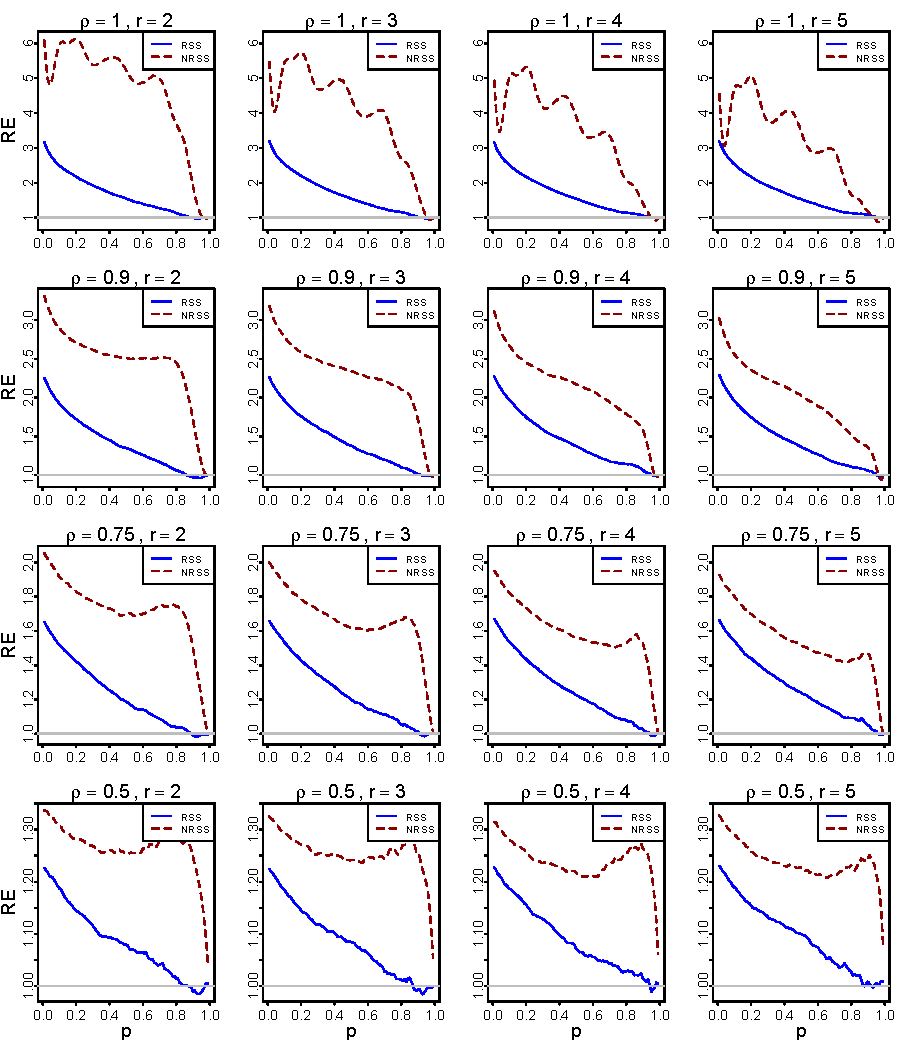
\includegraphics[scale=0.87]{Images/RE_m8_Gamma2}
	\vspace{-0.2cm}
	\caption{\footnotesize Simulated efficiencies of $m_{rss}$ (blue solid line) and $m_{nrss}$ (dark-red dash line) with respect to $m_{srs}$ as a function of $\rm{p}\in \{0.01,...,0.99\}$, for $\rm{G}(2)$ distribution,   with  $\rho  \in \left\lbrace 1,0.9,0.75,0.5 \right\rbrace$,  $r \in \left\lbrace 2,3,4,5 \right\rbrace$, and $m=8$.}
	\label{Fig1}
\end{figure}

\begin{figure}[h]
	\centering
	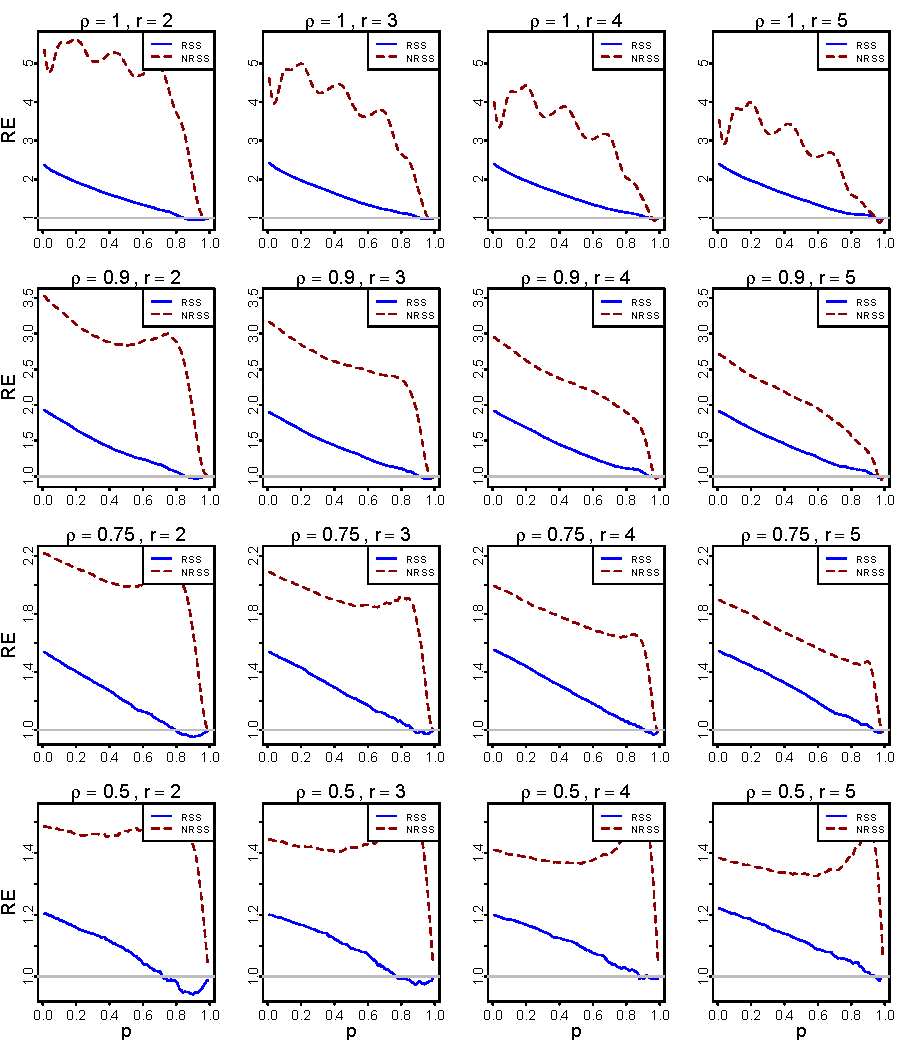
\includegraphics[scale=0.87]{Images/RE_m8_Gamma0.5}
	\vspace{-0.2cm}
	\caption{\footnotesize Simulated efficiencies of $m_{rss}$ (blue solid line) and $m_{nrss}$ (dark-red dash line) with respect to $m_{srs}$ as a function of $\rm{p}\in \{0.01,...,0.99\}$, for $\rm{G}(0.5)$ distribution,    with  $\rho  \in \left\lbrace 1,0.9,0.75,0.5 \right\rbrace$,  $r \in \left\lbrace 2,3,4,5 \right\rbrace$, and $m=8$.}
	\label{Fig2}
\end{figure}

\begin{figure}[h]
	\centering
	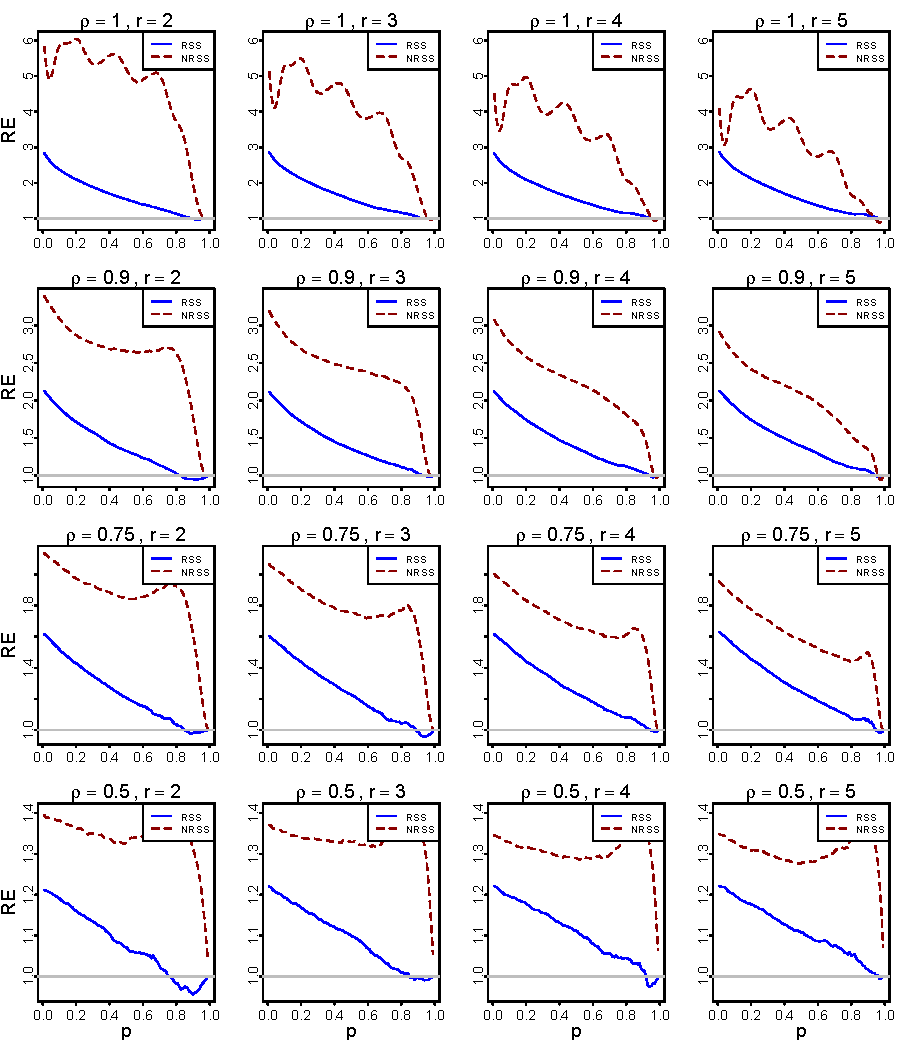
\includegraphics[scale=0.87]{Images/RE_m8_Exp1}
	\vspace{-0.2cm}
	\caption{\footnotesize Simulated efficiencies of $m_{rss}$ (blue solid line) and $m_{nrss}$ (dark-red dash line) with respect to $m_{srs}$ as a function of $\rm{p}\in \{0.01,...,0.99\}$, for $\rm{E}(1)$ distribution,    with  $\rho  \in \left\lbrace 1,0.9,0.75,0.5 \right\rbrace$,  $r \in \left\lbrace 2,3,4,5 \right\rbrace$, and $m=8$.}
	\label{Fig3}
\end{figure}

\section*{Discussion and Conclusion} 
In this paper, we proposed a nonparametric  estimator of the mean resitual life (MRL)  based on neoteric
ranked set sampling (NRSS), a modification of ranked  set sampling (RSS). We compared the performance of the proposed estimator
with its counterparts in  RSS and  simple random sampling (SRS) through a Monte Carlo simulation study. Our results showed that NRSS estimator outperforms its counterparts in most cases.

\begin{thebibliography}{6}
\bibitem[Frey(2012)]{Frey2012}
Frey, J. (2012). Constrained nonparametric estimation of the mean and the CDF using ranked-set sampling with a covariate. {\it Annals of the Institute of Statistical Mathematics}, 64(2), 439-456.

\bibitem[McIntyre(1952)]{McIntyre(1952)}
McIntyre, G. A. (1952). A method for unbiased selective sampling, using ranked sets. Australian journal of agricultural research, 3(4), 385-390.

\bibitem[Strzalkowska and Mahdizadeh(2014)]{Strzalkowska2014}
Strzalkowska-Kominiak, E., and Mahdizadeh, M. (2014). On the Kaplan-Meier estimator based on ranked set samples. {\it Journal of Statistical Computation and Simulation}, 84(12), 2577-2591.

\bibitem[Zamanzade and Al-Omari(2016)]{Zamanzade2016}
Zamanzade, E., and Al-Omari, A. I. (2016). New ranked set sampling for estimating the population mean and variance. {\it Hacettepe Journal of Mathematics and Statistics}, 45(6), 1891-1905.

\bibitem[Zamanzade et al.(2019)]{Zamanzade2019}
Zamanzade, E., Parvardeh, A., and Asadi, M. (2019). Estimation of mean residual life based on ranked set sampling. {\it Computational Statistics and Data Analysis}, 135, 35-55.

\bibitem[Zamanzade et al.(2020)]{Zamanzade2020}
Zamanzade, E., and Mahdizadeh, M. (2020). Using ranked set sampling with extreme ranks in estimating the population proportion. {\it Statistical methods in medical research}, 29(1), 165-177.


\end{thebibliography}
 \end{document}

